\documentclass{article}

\usepackage{format}

\usepackage[utf8]{inputenc}
\usepackage[T1]{fontenc}
\usepackage{hyperref}
\usepackage{url}
\usepackage{booktabs}
\usepackage{amsfonts}
\usepackage{nicefrac}
\usepackage{microtype}
\usepackage[usenames,dvipsnames]{xcolor}
\usepackage{graphicx}
\usepackage{multirow}
\usepackage{subfigure}
\usepackage{amssymb,amsmath}
\usepackage{amsthm}
\usepackage{float}
\usepackage{algorithm}
\usepackage{algorithmic}
\usepackage{thm-restate}
\usepackage{wrapfig}

\newtheorem{theorem}{Theorem}
\newtheorem{lemma}[theorem]{Lemma}
\newtheorem{proposition}[theorem]{Proposition}
\newtheorem{corollary}[theorem]{Corollary}
\newtheorem{definition}{Definition}
\newtheorem{remark}{Remark}
\newtheorem{assumption}{Assumption}

\newcommand{\R}{\mathbb{R}}
\newcommand{\E}{\mathbb{E}}
\renewcommand{\Pr}{\mathrm{Pr}}
\newcommand{\TV}{\mathrm{TV}}
\newcommand{\KL}{\mathrm{KL}}
\newcommand{\bH}{\bar{H}}
\newcommand{\ba}{\bar{a}}
\newcommand{\cT}{\mathcal{T}}
\newcommand{\cS}{\mathcal{S}}
\newcommand{\cF}{\mathcal{F}}
\newcommand{\cQ}{\mathcal{Q}}
\newcommand{\cA}{\mathcal{A}}
\newcommand{\ind}{\mathbf{1}}


\title{Reach-Avoid Constrained Selection for Safe Counterfactual Intervention Planning}


\author{%
  Anisio Lacerda \\
  Department of Computer Science\\
  Federal University of Minas Gerais\\
  Belo Horizonte, MG 30170-901 \\
  \texttt{anisio@dcc.ufmg.br} \\
}


\begin{document}

\maketitle

\begin{abstract}
Variational counterfactual intervention planning selects treatment sequences by optimizing an evidence lower bound (ELBO) toward a point target outcome. In clinical practice, however, the goal is typically to bring a patient's state into an \emph{acceptable range} while maintaining \emph{safety constraints} at every intermediate step---requirements that point-target optimization does not address. We introduce \emph{reach-avoid constrained selection}, a post-hoc method that filters ELBO-ranked candidate sequences through a reach-avoid feasibility criterion: the terminal outcome must lie within a target set~$\cT$ and all intermediate outcomes must remain within a safety set~$\cS$. We prove that reach-avoid ranking is more robust to variational approximation error than point-target ELBO ranking, with an explicit bound relating the ranking preservation margin to the variational gap~$\varepsilon_{\mathrm{VI}}$ and soft-indicator approximation error~$\varepsilon_{\mathrm{soft}}$. Empirically, on a cancer tumor growth simulator with known counterfactuals, reach-avoid constrained selection improves safety by 18--33 percentage points under moderate-to-strong confounding at modest ranking cost, Pareto-dominates soft-constraint alternatives, and transfers to all baseline models without retraining. On MIMIC-III intensive care data, the method lifts in-target diastolic blood pressure rates from 73--81\% to 99--100\%. The approach requires no model modification, no retraining, and is compatible with any variational counterfactual planner.
\end{abstract}


%% ============================================================
\section{Introduction}
\label{sec:intro}

Individualized treatment planning from observational data is a central challenge in precision medicine~\citep{chakraborty2014dynamic, murphy2003optimal}. Given a patient's clinical history, the goal is to recommend a sequence of interventions---medications, dosages, ventilation settings---that will produce the best outcome over a planning horizon~$\tau$. Recent advances in variational latent-dynamics models have made this tractable: Variational Counterfactual Intervention Planning \citep[VCIP;][]{melnychuk2025vcip} learns a latent state-space model from observational trajectories and selects treatment sequences by optimizing an evidence lower bound (ELBO) toward a target outcome value.

However, clinical treatment planning has two features that point-target ELBO optimization does not capture:

\paragraph{Range targets, not point targets.} Clinicians do not aim for a single number. They aim for an \emph{acceptable range}: diastolic blood pressure in $[60, 90]$~mmHg, tumor volume below a stage-dependent threshold, blood glucose within safe bounds. A treatment plan that overshoots the target by 1\% and one that undershoots it by 50\% receive the same ELBO penalty if they are equidistant from the point target, yet their clinical implications differ fundamentally. This limitation was explicitly identified in the VCIP peer review process, where a reviewer noted the restrictive nature of single-point targets for clinical applications and the authors acknowledged range-based targets as important future work.

\paragraph{Path safety, not just terminal achievement.} ELBO-based planning evaluates only the terminal outcome~$Y_{t+\tau}$. It is blind to what happens along the way. A chemotherapy regimen that produces dangerously high toxicity at step~$t{+}3$ before recovering at step~$t{+}\tau$ may rank identically to a safe regimen---both achieve the same terminal tumor volume. In clinical practice, intermediate safety violations are unacceptable: a patient whose blood pressure drops to dangerous levels during treatment has suffered harm regardless of the final reading.

These concerns arise naturally from the reach-avoid control literature~\citep{mitchell2005reach, fisac2015reach}, where the objective is to steer a dynamical system into a target set while avoiding unsafe regions throughout the trajectory. Figure~\ref{fig:concept} illustrates the distinction: ELBO-based selection picks the sequence with the best terminal loss (D), ignoring its unsafe intermediate path, while reach-avoid constrained selection picks the best ELBO among sequences with safe trajectories (A).

\begin{figure}[t]
\centering
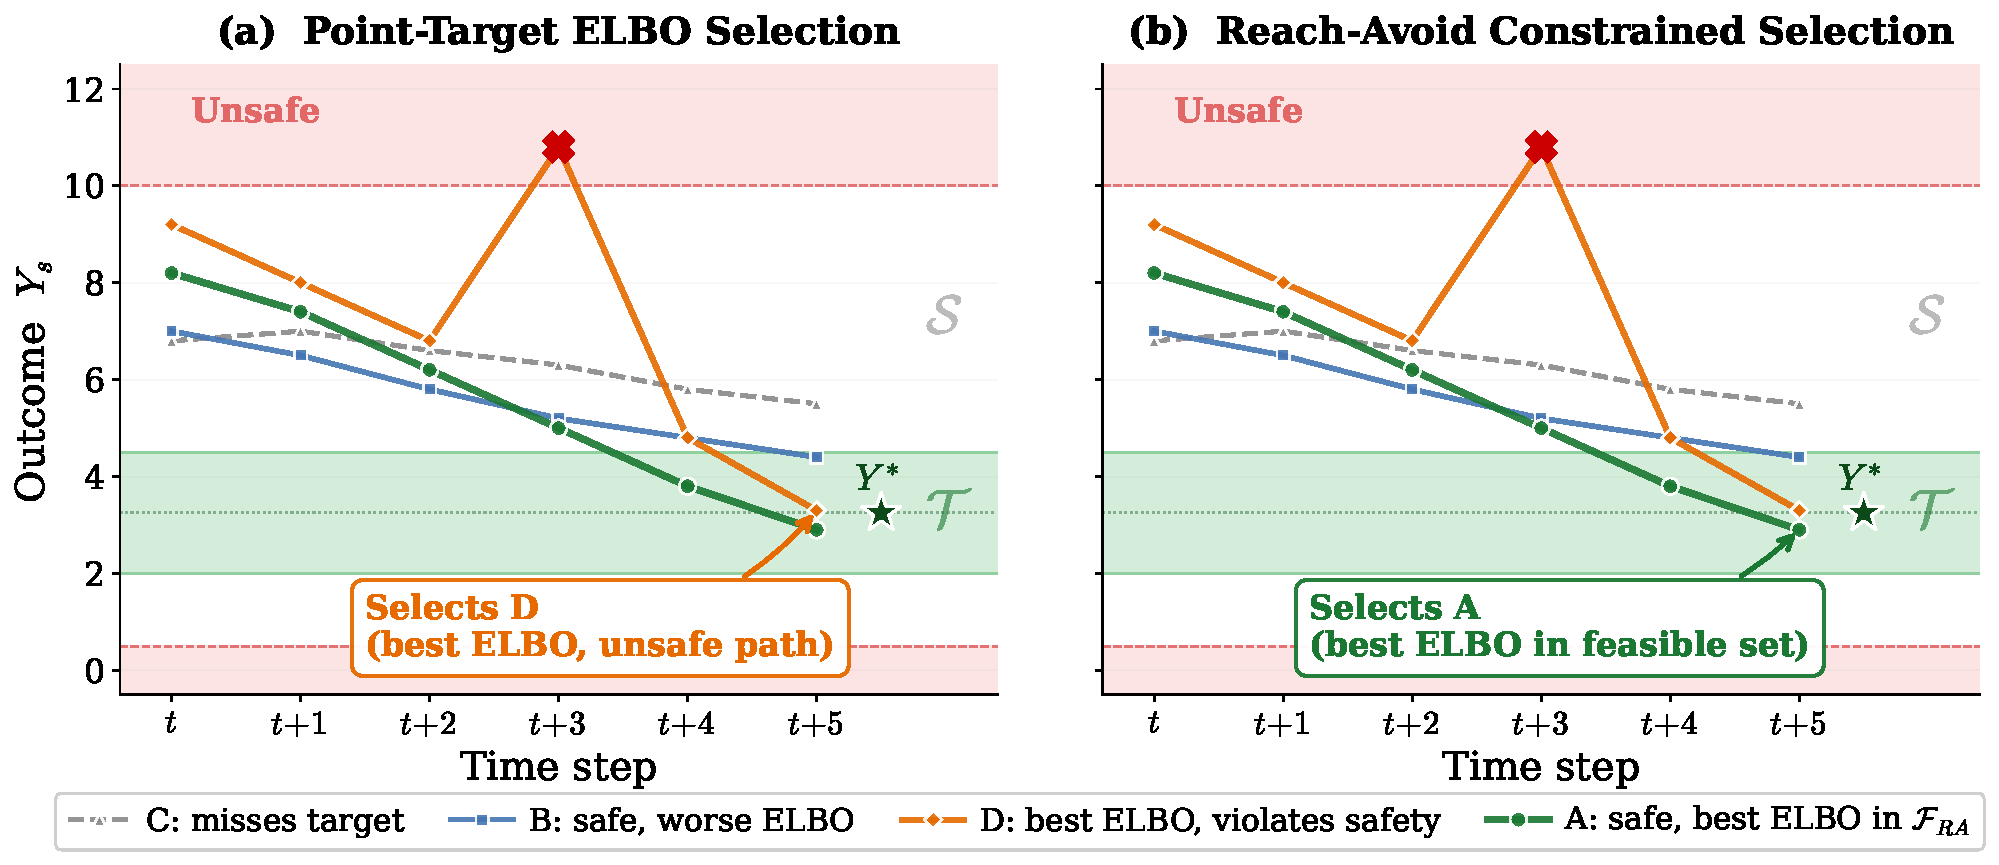
\includegraphics[width=\textwidth]{../lightning-hydra-template-main/src/reach_avoid/figures/rc7_figure1_concept.pdf}
\caption{\textbf{Reach-avoid vs.\ point-target selection.} The dark green star~($\bigstar$) marks the ELBO point target~$Y^*$. Left: ELBO-based selection picks sequence D (closest to $Y^*$ at terminal time) despite its safety violation at $t{+}3$. Right: RA-constrained selection restricts to feasible sequences (those reaching $\cT$ while staying in $\cS$) and selects the best ELBO among them (A over B, which is also feasible but has worse ELBO). D is rejected for violating safety; C for missing the target.}
\label{fig:concept}
\end{figure}

\paragraph{Our approach.} We propose \emph{reach-avoid constrained selection}: given a set of candidate treatment sequences ranked by ELBO, we filter out sequences that fail a reach-avoid feasibility criterion and select the best ELBO among the feasible set:
\begin{equation}
\label{eq:ra_selection}
\ba^* = \arg\min_{\ba \in \cF_{\mathrm{RA}}} \mathrm{ELBO}(\ba),
\end{equation}
where $\cF_{\mathrm{RA}} = \{\ba : Y_{t+\tau}[\ba] \in \cT \text{ and } Y_s[\ba] \in \cS \text{ for all } s = t, \ldots, t{+}\tau\}$ is the set of reach-avoid feasible sequences. This is deliberately simple: no new model, no retraining, no gradient-based planning. The method operates as a \emph{post-hoc safety filter} on any existing variational counterfactual planner.

The simplicity is a feature. By separating safety (via the RA filter) from quality (via ELBO ranking), we avoid the failure mode we observed when attempting to use RA scoring as a \emph{replacement} for ELBO ranking: the RA score is near-binary (sequences are either clearly feasible or clearly not), providing no discrimination among candidates. ELBO ranking and RA feasibility are complementary---each does what the other cannot.

\paragraph{Contributions.}
\begin{enumerate}
\item \textbf{Problem formulation.} We formalize reach-avoid counterfactual intervention planning, connecting the clinical requirement of range targets with path safety to the reach-avoid framework from control theory (Section~\ref{sec:method}).
\item \textbf{Ranking robustness theory.} We prove that reach-avoid ranking is more robust to variational approximation error than point-target ELBO ranking (Theorem~\ref{thm:ranking_robustness}), with an explicit bound on the ranking preservation margin. We empirically verify the bound is non-vacuous with $\varepsilon_{\mathrm{VI}} \approx 0.09$--$0.23$ (Section~\ref{sec:theory}).
\item \textbf{Comprehensive experiments.} On the Cancer simulator with known counterfactuals, reach-avoid constrained selection yields $+$18--33 percentage point (pp) safety improvement under moderate-to-strong confounding, Pareto-dominates soft-constraint alternatives, and generalizes across five baseline models without retraining. On MIMIC-III ICU data, it lifts in-target rates from 73--81\% to 99--100\% (Section~\ref{sec:experiments}).
\item \textbf{Model-agnostic post-hoc method.} The approach requires no retraining---we show empirically that RA-aware retraining produces identical results to post-hoc filtering---and is compatible with any variational counterfactual planner (Section~\ref{sec:retraining_result}).
\end{enumerate}


%% ============================================================
\section{Related Work}
\label{sec:related}

We provide a concise overview here; Appendix~\ref{app:extended_related_work} contains a comprehensive survey with additional references.

\paragraph{Counterfactual outcome estimation and planning.} A growing body of work estimates individualized treatment effects from longitudinal observational data, including balanced representations~\citep{shalit2017estimating, bica2020crn}, variational approaches~\citep{louizos2017cevae}, attention-based architectures~\citep{melnychuk2022causal}, recurrent methods~\citep{lim2018forecasting, li2021gnet}, continuous-time models~\citep{seedat2022actin}, and synthetic control~\citep{qian2021synctwin}. Recent advances address hidden confounding~\citep{bica2020tsd, frauen2023sharp} and employ contrastive~\citep{kim2024causalcpc} or generative~\citep{wu2024counterfactual, pawlowski2020deep} approaches. These methods estimate outcomes for \emph{given} treatments but do not optimize over treatment sequences. VCIP~\citep{melnychuk2025vcip} extends this line to \emph{planning}: it selects intervention sequences by ELBO minimization toward a point target. Our work keeps the VCIP planning infrastructure intact and adds a safety-aware selection layer.

\paragraph{Dynamic treatment regimes.} The DTR literature~\citep{murphy2003optimal, chakraborty2014dynamic, hernan2020causal} formalizes sequential treatment decisions under the potential outcomes framework, with recent work on when-to-treat policies~\citep{nie2021learning} and batch constrained learning~\citep{le2019batch}. Most DTR methods learn decision rules mapping states to actions, optimizing expected outcomes over the full trajectory. In contrast, VCIP and our extension operate in a \emph{counterfactual planning} mode: given a specific patient history, they evaluate and rank complete intervention sequences. The reach-avoid formulation adds the constraint that trajectories must remain safe---a concern shared with constrained DTR work but addressed here through a distinct mechanism (post-hoc filtering rather than constrained policy learning).

\paragraph{Safe and constrained sequential decision-making.} Safe reinforcement learning~\citep{garcia2015comprehensive, achiam2017constrained, tessler2019rcpo} constrains policies to satisfy safety specifications during execution, from Lyapunov-based methods~\citep{chow2018safe} to safety layers~\citep{dalal2018safe} to offline safe RL~\citep{zheng2024fisor}. These methods operate in the online or offline RL setting, requiring either environment interaction or fixed datasets of state-action trajectories. Our setting is fundamentally different: we select among candidate plans evaluated on a learned model, with no opportunity for policy-level correction. This distinction motivates a filter-based approach rather than constrained policy optimization. The \emph{reach-avoid} concept from control theory~\citep{mitchell2005reach, fisac2015reach, bansal2021deepreach} formalizes the objective of reaching a target set while avoiding unsafe regions. We import this concept into the variational counterfactual planning framework, replacing the continuous reachability computation with a discrete feasibility check over candidate sequences.

\paragraph{Variational causal inference.} CEVAE~\citep{louizos2017cevae} pioneered VAE-based causal inference under hidden confounding; Deep SCMs~\citep{pawlowski2020deep} extended this to full counterfactual reasoning via normalizing flows. VCI~\citep{wu2025vci} derives an ELBO for individual-level counterfactual likelihoods in a static setting, introducing latent disentanglement via $D_{\KL}[q(z|y,t,x) \| q(z|y',t',x)]$. We draw on VCI's insight that latent action-sensitivity is a diagnostic for counterfactual model quality (Section~\ref{sec:e4_diagnostic}), adapting it to the sequential setting. Our diagnostic reveals that VCIP's latent space is nearly action-invariant ($D_{\KL} \approx 10^{-5}$), with action-outcome coupling residing entirely in the decoder.


%% ============================================================
\section{Background: Variational Counterfactual Intervention Planning}
\label{sec:background}

We briefly review the VCIP framework~\citep{melnychuk2025vcip} to establish notation.

\paragraph{Setting.} Consider a longitudinal observational dataset with patient histories $\bH_t = (X_1, A_1, Y_1, \ldots, X_t, A_t, Y_t)$, where $X_s \in \R^p$ are time-varying covariates, $A_s \in \cA$ are treatments (binary or categorical), and $Y_s \in \R^d$ are outcomes of interest. Given a patient's history $\bH_t$ up to time $t$ and a planning horizon $\tau$, the goal is to select an intervention sequence $\ba = (a_{t+1}, \ldots, a_{t+\tau}) \in \cA^\tau$ that optimizes the counterfactual outcome $Y_{t+\tau}[\ba]$.

\paragraph{Latent dynamics model.} VCIP posits a latent state $Z_s \in \R^{d_z}$ with:
\begin{itemize}
    \item Generative transition: $p_\theta(Z_{s+1} \mid Z_s, a_s)$, modeling how latent states evolve under treatment,
    \item Emission (decoder): $p_\theta(Y_s \mid Z_s)$, mapping latent states to predicted outcomes,
    \item Variational posterior: $q_\phi(Z_{t:t+\tau} \mid \bH_t, \ba)$, approximating the intractable posterior over latent trajectories.
\end{itemize}
The model is trained by maximizing an ELBO on observed trajectories:
\begin{equation}
\label{eq:elbo}
\mathcal{L}(\theta, \phi) = \E_{q_\phi}\!\left[\sum_{s=t+1}^{t+\tau} \log p_\theta(Y_s \mid Z_s)\right] - D_{\KL}\!\left[q_\phi(Z_{t:t+\tau} \mid \bH_t, \ba) \,\|\, p_\theta(Z_{t:t+\tau} \mid \bH_t, \ba)\right].
\end{equation}

\paragraph{Planning by ELBO minimization.} Given a patient history $\bH_t$, VCIP generates $k$ candidate treatment sequences (via perturbation of the observed treatments) and selects the one minimizing the ELBO loss with respect to a point target $Y^*$:
\begin{equation}
\label{eq:vcip_selection}
\ba^*_{\mathrm{ELBO}} = \arg\min_{\ba \in \{\ba_1, \ldots, \ba_k\}} \mathrm{ELBO}(\ba; \bH_t, Y^*).
\end{equation}
The ELBO loss decomposes into a reconstruction term (how well the predicted outcome matches $Y^*$) and a KL regularization term. This formulation ranks sequences by how well the variational model predicts they will achieve the point target. The key limitation is that $Y^*$ is a single point, and only the terminal step $s = t + \tau$ contributes to the ranking---intermediate outcomes are ignored.


%% ============================================================
\section{Method: Reach-Avoid Constrained Selection}
\label{sec:method}

\subsection{Reach-Avoid Feasibility}
\label{sec:ra_feasibility}

\begin{definition}[Reach-Avoid Event]
\label{def:ra_event}
Given a target set $\cT \subseteq \R^d$ for the terminal outcome and a safety set $\cS \subseteq \R^d$ for intermediate outcomes, the \emph{reach-avoid event} for intervention sequence $\ba$ is:
\begin{equation}
E(\ba) := \{Y_{t+\tau}[\ba] \in \cT\} \cap \bigcap_{s=t}^{t+\tau} \{Y_s[\ba] \in \cS\}.
\end{equation}
\end{definition}

The event $E(\ba)$ requires the terminal outcome to land in the target set (\emph{reach}) while all intermediate outcomes remain in the safety set (\emph{avoid} unsafe regions). The sets $\cT$ and $\cS$ encode domain knowledge:
\begin{itemize}
    \item \textbf{Cancer:} $\cT = \{y : \text{tumor volume} \leq 3.0\}$ (clinically manageable stage), $\cS = \{y : \text{volume} \leq 12.0\} \cap \{y : \text{chemo dosage} \leq 5.0\}$ (no tumor explosion, no toxic chemotherapy).
    \item \textbf{ICU (MIMIC-III):} $\cT = \{y : \text{DBP} \in [60, 90] \text{ mmHg}\}$ (normotensive range), $\cS = \{y : \text{DBP} \in [40, 120] \text{ mmHg}\}$ (avoids dangerous hypo-/hypertension).
\end{itemize}

\subsection{Soft Indicators}
\label{sec:soft_indicators}

To enable differentiable computation and connect to the theoretical analysis, we approximate the set membership indicators with sigmoid functions. For an upper-bounded constraint $y \leq u$:
\begin{equation}
g_u(y; \kappa) = \sigma(\kappa(u - y)),
\end{equation}
where $\sigma$ is the logistic sigmoid and $\kappa > 0$ controls hardness. For an interval constraint $y \in [\ell, u]$:
\begin{equation}
g_{[\ell, u]}(y; \kappa) = \sigma(\kappa(y - \ell)) \cdot \sigma(\kappa(u - y)).
\end{equation}
The \emph{reach-avoid score} for a candidate sequence $\ba$ is then:
\begin{equation}
\label{eq:ra_score}
J_{\mathrm{RA}}(\ba) = g_{\cT}(Y_{t+\tau}[\ba]) \cdot \prod_{s=t}^{t+\tau} g_{\cS}(Y_s[\ba]).
\end{equation}
A sequence is \emph{feasible} if $J_{\mathrm{RA}}(\ba) \geq \delta$ for a threshold $\delta \in (0, 1)$. In the hard-filter limit ($\kappa \to \infty$), this reduces to the indicator $\ind\{E(\ba)\}$. Our experiments show that $\kappa \geq 5$ is indistinguishable from the hard filter ($>99.9\%$ selection agreement; see Section~\ref{sec:ablation_kappa}).

\subsection{Constrained Selection}
\label{sec:constrained_selection}

Given $k$ candidate sequences $\{\ba_1, \ldots, \ba_k\}$ ranked by ELBO, the \emph{reach-avoid constrained selection} rule is:
\begin{equation}
\label{eq:constrained}
\ba^* = \arg\min_{\ba \in \cF_{\mathrm{RA}}} \mathrm{ELBO}(\ba; \bH_t, Y^*),
\quad \text{where } \cF_{\mathrm{RA}} = \{\ba_i : J_{\mathrm{RA}}(\ba_i) \geq \delta\}.
\end{equation}
If $\cF_{\mathrm{RA}} = \emptyset$ (no feasible sequence), we fall back to unconstrained ELBO selection~\eqref{eq:vcip_selection}. The full procedure is summarized in Algorithm~\ref{alg:ra_selection}.

\begin{algorithm}[t]
\caption{Reach-Avoid Constrained Selection}
\label{alg:ra_selection}
\begin{algorithmic}[1]
\REQUIRE Patient history $\bH_t$, trained model $(p_\theta, q_\phi)$, target set $\cT$, safety set $\cS$, candidates $k$, hardness $\kappa$, threshold $\delta$
\STATE Generate $k$ candidate sequences $\{\ba_1, \ldots, \ba_k\}$ via treatment perturbation
\STATE Compute $\mathrm{ELBO}(\ba_i; \bH_t, Y^*)$ for each $i$ using the variational model
\STATE Obtain outcome trajectories $\{Y_s[\ba_i]\}_{s=t}^{t+\tau}$ for each $i$ \COMMENT{simulator or model predictions}
\STATE Compute RA scores: $J_{\mathrm{RA}}(\ba_i) \gets g_\cT(Y_{t+\tau}[\ba_i]) \cdot \prod_s g_\cS(Y_s[\ba_i])$
\STATE Filter: $\cF_{\mathrm{RA}} \gets \{\ba_i : J_{\mathrm{RA}}(\ba_i) \geq \delta\}$
\IF{$\cF_{\mathrm{RA}} \neq \emptyset$}
    \RETURN $\ba^* = \arg\min_{\ba \in \cF_{\mathrm{RA}}} \mathrm{ELBO}(\ba)$
\ELSE
    \RETURN $\ba^* = \arg\min_{\ba \in \{\ba_1, \ldots, \ba_k\}} \mathrm{ELBO}(\ba)$ \COMMENT{fallback}
\ENDIF
\end{algorithmic}
\end{algorithm}

\begin{remark}[Why hard filtering, not soft penalty]
\label{rem:hard_vs_soft}
An alternative is Lagrangian relaxation: $\min_{\ba} \mathrm{ELBO}(\ba) + \lambda (1 - J_{\mathrm{RA}}(\ba))$. We found empirically that hard filtering Pareto-dominates the soft penalty at high safety levels (Section~\ref{sec:soft_vs_hard}). The key reason: a global penalty shifts rankings for \emph{all} sequences, degrading ELBO ranking quality among safe candidates. Hard filtering is surgical---it removes infeasible sequences while preserving the ELBO ranking among the feasible set. This observation also has a theoretical basis: within $\cF_{\mathrm{RA}}$, the ELBO ranking is unperturbed, so the constrained selection inherits the full ranking quality of the base model.
\end{remark}


%% ============================================================
\section{Theory: Ranking Robustness}
\label{sec:theory}

We now establish that reach-avoid ranking is provably more robust to variational approximation error than point-target ELBO ranking. The key insight is that set membership is a \emph{coarsening} of continuous outcomes: many different outcome values map to the same feasibility verdict, making the ranking less sensitive to small perturbations in the variational approximation.

\begin{assumption}[Bounded variational gap]
\label{ass:vi_gap}
For any intervention sequence $\ba$, the total variation distance between the true outcome distribution $p_\theta(\cdot \mid \ba, \bH_t)$ and the variational approximation $q_\phi(\cdot \mid \ba, \bH_t)$ is bounded:
\begin{equation}
\TV(p_\theta(\cdot \mid \ba, \bH_t),\; q_\phi(\cdot \mid \ba, \bH_t)) \leq \varepsilon_{\mathrm{VI}}.
\end{equation}
\end{assumption}

\begin{assumption}[Bounded soft-indicator error]
\label{ass:soft_error}
The soft indicator $g_\cT$ approximates the true indicator $\ind_\cT$ with bounded error:
$\|g_\cT - \ind_\cT\|_\infty \leq \varepsilon_{\mathrm{soft}}(\kappa)$,
where $\varepsilon_{\mathrm{soft}}(\kappa) \to 0$ as $\kappa \to \infty$. Similarly for $g_\cS$.
\end{assumption}

Assumption~\ref{ass:vi_gap} is standard in variational inference analysis. Assumption~\ref{ass:soft_error} is constructive: for the logistic sigmoid with hardness $\kappa$, $\varepsilon_{\mathrm{soft}}(\kappa) = \sigma(0) = 0.5$ at the boundary, but this worst case occurs on a measure-zero set. We verify empirically that $\kappa \geq 5$ yields effectively zero approximation error (Section~\ref{sec:ablation_kappa}).

\begin{definition}[Reach-avoid probability]
For an intervention sequence $\ba$, the \emph{true reach-avoid probability} under the model is:
\begin{equation}
P(\ba) := \E_{p_\theta}\left[\ind\{Y_{t+\tau} \in \cT\} \cdot \prod_{s=t}^{t+\tau} \ind\{Y_s \in \cS\} \;\middle|\; \bH_t, \ba\right].
\end{equation}
The \emph{approximate reach-avoid probability} under the variational posterior is $\hat{P}(\ba)$, defined analogously with $q_\phi$ replacing $p_\theta$ and soft indicators replacing hard indicators.
\end{definition}

\begin{theorem}[Ranking robustness of reach-avoid selection]
\label{thm:ranking_robustness}
Under Assumptions~\ref{ass:vi_gap} and~\ref{ass:soft_error}, for any two intervention sequences $\ba_1, \ba_2$:

\textbf{(a) RA ranking preservation.} If the true reach-avoid probability margin satisfies
\begin{equation}
\label{eq:ra_margin}
m_{\mathrm{RA}} := |P(\ba_1) - P(\ba_2)| > 2\varepsilon_{\mathrm{VI}} + 2(\tau+1)\varepsilon_{\mathrm{soft}}(\kappa),
\end{equation}
then the approximate ranking is preserved: $\hat{P}(\ba_1) > \hat{P}(\ba_2)$ iff $P(\ba_1) > P(\ba_2)$.

\textbf{(b) Point-target ranking threshold.} For point-target ELBO ranking, let $d(\ba) = \E_{p_\theta}[\|Y_{t+\tau}[\ba] - Y^*\|^2 \mid \bH_t, \ba]$ be the true expected squared distance to target. Ranking preservation requires:
\begin{equation}
\label{eq:elbo_margin}
m_{\mathrm{ELBO}} := |d(\ba_1) - d(\ba_2)| > 2\varepsilon_{\mathrm{VI}} \cdot C_d,
\end{equation}
where $C_d = \sup_{\ba} \mathrm{Var}_{p_\theta}(\|Y_{t+\tau}[\ba] - Y^*\|^2 \mid \bH_t, \ba)^{1/2}$ depends on the outcome variance.

\textbf{(c) Strict improvement.} When the boundary mass $\beta := \sup_{\ba} p_\theta(Y_{t+\tau}[\ba] \in \partial_\epsilon \cT \mid \bH_t, \ba)$ is small (most outcomes clearly inside or outside $\cT$), we have $m_{\mathrm{RA}} \gg m_{\mathrm{ELBO}} / C_d$, i.e., RA ranking is preserved for pairs where ELBO ranking would be inverted.
\end{theorem}

\begin{proof}[Proof sketch (full proof in Appendix~\ref{app:proofs})]
\textbf{Part (a):} The reach-avoid probability is a bounded functional ($P \in [0,1]$). By the variational characterization of total variation, $|P(\ba) - P_{q_\phi}(\ba)| \leq \varepsilon_{\mathrm{VI}}$. The soft-indicator approximation contributes at most $(\tau+1)\varepsilon_{\mathrm{soft}}$ error (one terminal gate plus $\tau$ safety gates). Triangle inequality gives $|\hat{P}(\ba) - P(\ba)| \leq \varepsilon_{\mathrm{VI}} + (\tau+1)\varepsilon_{\mathrm{soft}}$. Ranking preservation follows when the margin exceeds twice this error.

\textbf{Part (b):} The squared distance $\|Y - Y^*\|^2$ is unbounded, so the TV bound introduces a variance-dependent factor~$C_d$. In practice, $C_d$ is large when outcome distributions have high spread---precisely the regime where point-target ranking is most fragile.

\textbf{Part (c):} When most outcomes are unambiguously inside or outside $\cT$ (low boundary mass $\beta$), reach-avoid probabilities cluster near 0 or 1, giving large margins $m_{\mathrm{RA}} \approx 1$. Meanwhile, point distances can be nearly identical for outcomes on opposite sides of the target boundary, giving $m_{\mathrm{ELBO}} \approx 0$.
\end{proof}

\begin{corollary}
\label{cor:hard_filter_exact}
In the hard-filter limit ($\kappa \to \infty$, so $\varepsilon_{\mathrm{soft}} = 0$), reach-avoid ranking is preserved whenever $|P(\ba_1) - P(\ba_2)| > 2\varepsilon_{\mathrm{VI}}$. For deterministic trajectories (as in the Cancer simulator), feasibility is binary ($P \in \{0, 1\}$), so the filter is exact whenever $\varepsilon_{\mathrm{VI}} < 0.5$.
\end{corollary}

\paragraph{Empirical verification.} We estimate $\varepsilon_{\mathrm{VI}}$ on the Cancer simulator using rank mean absolute error as a proxy (Section~\ref{sec:ablation_eps}). We find $\varepsilon_{\mathrm{VI}} \approx 0.09$--$0.23$ across confounding strengths, with ELBO pairwise ranking preservation at 61--87\%. The bound is non-vacuous: for pairs differing in feasibility status (margin $= 1$), the condition $m > 2\varepsilon_{\mathrm{VI}} \approx 0.18$--$0.46$ is easily satisfied. Notably, $\varepsilon_{\mathrm{VI}}$ \emph{decreases} with confounding strength $\gamma$ (the model is better calibrated when treatment effects are stronger), meaning the bound is tightest precisely where RA filtering is most valuable.


%% ============================================================
\section{Experiments}
\label{sec:experiments}

We evaluate reach-avoid constrained selection on two datasets: (1)~a cancer tumor growth simulator~\citep{bica2020cancer} where ground-truth counterfactual trajectories are available, and (2)~MIMIC-III intensive care data~\citep{johnson2016mimic} where only observed outcomes are available.

\subsection{Setup}
\label{sec:setup}

\paragraph{Cancer simulator.} The simulator models tumor growth under chemotherapy and radiotherapy~\citep{geng2017cancer, bica2020cancer}. Treatment assignment is confounded by a parameter $\gamma \in \{1, 2, 3, 4\}$: higher $\gamma$ means patients with larger tumors receive more aggressive treatment, creating stronger confounding between treatment assignment and outcomes. We use the VCIP~\citep{melnychuk2025vcip} implementation with 5 random seeds per configuration, $k = 100$ candidate sequences per patient, $n = 100$ evaluation patients, and planning horizons $\tau \in \{2, 4, 6, 8\}$.

\paragraph{Cancer thresholds.} Calibrated from the data distribution: target set $\cT$: tumor volume $\leq 3.0$ (below the 60th percentile, corresponding to a clinically manageable stage). Safety set $\cS$: tumor volume $\leq 12.0$ (below the 95th percentile) and chemotherapy dosage $\leq 5.0$ (below the toxic threshold) at all intermediate steps.

\paragraph{MIMIC-III.} We use the MIMIC-Extract pipeline~\citep{wang2020mimic} to extract 34,472 ICU patients with hourly measurements from the MIMIC-III database~\citep{johnson2016mimic}. The outcome is diastolic blood pressure (DBP). Target set: DBP $\in [60, 90]$~mmHg (normotensive range). Safety set: DBP $\in [40, 120]$~mmHg at all steps (avoids dangerous hypo-/hypertension). We train VCIP models with 5 seeds and evaluate with $\tau \in \{2, 3, 4, 5\}$.

\paragraph{Baselines.} We compare five counterfactual estimation models, each evaluated with and without RA-constrained selection: VCIP~\citep{melnychuk2025vcip}, CRN~\citep{bica2020crn}, Causal Transformer (CT)~\citep{melnychuk2022causal}, RMSN~\citep{lim2018forecasting}, and ACTIN~\citep{seedat2022actin}.

\paragraph{Metrics.} (1)~\emph{GRP}: ground-truth rank percentile of the selected sequence among $k$ candidates (higher = better; available on Cancer only). (2)~\emph{Top-1 accuracy}: fraction of patients for whom the selected sequence is the ground-truth best. (3)~\emph{Safety rate}: fraction where all intermediate safety constraints hold. (4)~\emph{In-target rate}: fraction where the terminal outcome lies in $\cT$. (5)~\emph{Feasibility}: fraction of candidate sequences passing the RA filter.


\subsection{Main Results: Cancer Simulator}
\label{sec:cancer_results}

Table~\ref{tab:main_cancer} presents the core results at $\gamma = 4$ (strongest confounding), where the benefit of RA-constrained selection is most pronounced.

\begin{table}[t]
\centering
\caption{Reach-avoid constrained selection on Cancer ($\gamma = 4$, mean $\pm$ std across 5 seeds). ``ELBO'' = unconstrained ELBO selection. ``RA'' = reach-avoid constrained ELBO selection.}
\label{tab:main_cancer}
\small
\begin{tabular}{l c c c c c c c}
\toprule
$\tau$ & Feas.\% & ELBO Top-1 & RA Top-1 & ELBO Safe & RA Safe & ELBO In-T & RA In-T \\
\midrule
2 & 53.6 & 18.8\% & 17.4\% & 85.0\% & 94.4\% & 85.0\% & 94.4\% \\
4 & 29.7 & 42.4\% & 39.4\% & 84.6\% & 95.6\% & 84.6\% & 95.6\% \\
6 & 16.8 & 62.6\% & 54.2\% & 84.8\% & 96.2\% & 84.8\% & 96.2\% \\
8 & 10.3 & 75.8\% & 60.4\% & 85.6\% & 97.0\% & 85.6\% & 97.0\% \\
\bottomrule
\end{tabular}
\end{table}

RA-constrained selection consistently improves safety and in-target rates by 9--12~pp across all horizons, at the cost of 1--15~pp in Top-1 accuracy. The trade-off is most favorable at shorter horizons ($\tau = 2$: $+$9.4~pp safety for $-$1.4~pp Top-1) where feasibility is highest (54\%), and becomes more aggressive at longer horizons where fewer candidates pass intermediate safety across all steps.

\paragraph{Confounding strength sensitivity.} Table~\ref{tab:gamma_sweep} shows results across all $\gamma$ values. At $\gamma = 1$ (weak confounding), the constraint is nearly a no-op---ELBO already selects safe plans. At $\gamma = 4$, the benefit is substantial: $+$10.8~pp in-target gain, $+$15.2~pp safety gain. The method never hurts: worst-case Top-1 cost is 7~pp with 15~pp safety gain.

\begin{table}[t]
\centering
\caption{RA-constrained selection across confounding strengths (averaged over $\tau \in \{2,4,6,8\}$, mean across 5 seeds). Safety and in-target gains are absolute pp differences vs.\ ELBO.}
\label{tab:gamma_sweep}
\small
\begin{tabular}{l c c c c c c c}
\toprule
$\gamma$ & GRP & ELBO Top-1 & RA Top-1 & $\Delta$Top-1 & Safety gain & In-T gain & Avg Feas \\
\midrule
1 & 0.757 & 5.3\% & 5.3\% & $+$0.0 pp & $+$21.3 pp & $+$0.2 pp & 20.2\% \\
2 & 0.889 & 18.8\% & 17.8\% & $-$1.0 pp & $+$14.8 pp & $+$1.2 pp & 22.7\% \\
3 & 0.940 & 36.4\% & 32.4\% & $-$4.0 pp & $+$11.8 pp & $+$3.9 pp & 26.0\% \\
4 & 0.963 & 49.9\% & 42.9\% & $-$7.0 pp & $+$15.2 pp & $+$10.8 pp & 27.6\% \\
\bottomrule
\end{tabular}
\end{table}

This gamma sweep also functions as a partial sensitivity analysis for the sequential ignorability assumption: as confounding strengthens, RA-constrained selection becomes more valuable, suggesting the method is robust to---and even benefits from---model misspecification due to unobserved confounding.


\subsection{MIMIC-III Results}
\label{sec:mimic_results}

On MIMIC-III (Table~\ref{tab:mimic}), RA-constrained selection lifts the in-target diastolic BP rate from 73--81\% to 99--100\% across all horizons. Feasibility decreases with $\tau$ (33\% $\to$ 22\%) as longer horizons have fewer sequences satisfying safety at every step.

\begin{table}[t]
\centering
\caption{MIMIC-III diastolic BP results (5 seeds pooled). Target: DBP $\in [60,90]$~mmHg. Safety: DBP $\in [40, 120]$~mmHg at all steps.}
\label{tab:mimic}
\small
\begin{tabular}{l c c c c c c}
\toprule
$\tau$ & Feas.\% & ELBO In-T & RA In-T & $\Delta$ In-T & ELBO DBP & RA DBP \\
\midrule
2 & 33.4\% & 73.0\% & 100.0\% & $+$27.0 pp & 60.4 mmHg & 61.3 mmHg \\
3 & 28.6\% & 79.2\% & 100.0\% & $+$20.8 pp & 60.6 mmHg & 61.6 mmHg \\
4 & 24.7\% & 80.0\% & 99.8\% & $+$19.8 pp & 60.7 mmHg & 61.8 mmHg \\
5 & 22.5\% & 81.2\% & 99.2\% & $+$18.0 pp & 60.8 mmHg & 61.8 mmHg \\
\bottomrule
\end{tabular}
\end{table}

RA-constrained selection also shifts predicted treatment patterns: constrained selections have substantially lower vasopressor rates (0.01--0.29 vs.\ 0.29--0.79 under ELBO), suggesting the constraint preferentially removes aggressive treatment plans that risk hypotension. While we cannot verify ground-truth safety on real data (counterfactual trajectories are unobservable), the treatment pattern shift is clinically plausible: lower vasopressor use is consistent with avoiding blood pressure drops.


\subsection{Model-Agnostic Evaluation}
\label{sec:model_agnostic}

A key claim is that RA-constrained selection works as a universal safety filter. Table~\ref{tab:model_agnostic} shows results across all five models at $\gamma = 4$, $\tau = 4$. Baseline models benefit \emph{more} from RA filtering than VCIP: their constrained average ranks improve by 13--15 positions (vs.\ a slight degradation for VCIP). This is because filtering removes a larger fraction of poor selections from weaker models.

\begin{table}[t]
\centering
\caption{Model-agnostic RA filtering ($\gamma = 4$, $\tau = 4$). Rank $\Delta$: change in average rank among 100 candidates (negative = improvement). RA filtering improves all models' safety rates.}
\label{tab:model_agnostic}
\small
\begin{tabular}{l c c c c c c}
\toprule
Model & GRP & ELBO Top-1 & RA Top-1 & ELBO Safe & RA Safe & Rank $\Delta$ \\
\midrule
VCIP  & 0.973 & 44.4\% & 39.4\% & 84.6\% & 95.6\% & $+$2.0 \\
ACTIN & 0.676 & 5.2\%  & 4.4\%  & 52.2\% & 75.8\% & $-$12.9 \\
CT    & 0.544 & 3.2\%  & 2.6\%  & 47.8\% & 69.8\% & $-$15.0 \\
CRN   & 0.690 & 6.0\%  & 5.2\%  & 53.4\% & 76.4\% & $-$12.9 \\
RMSN  & 0.578 & 2.8\%  & 2.0\%  & 49.0\% & 72.2\% & $-$13.2 \\
\bottomrule
\end{tabular}
\end{table}

This demonstrates that RA-constrained selection is truly model-agnostic: the safety filter operates on ground-truth trajectories (in the Cancer simulator), independent of which model provides the ELBO ranking. Any model---no matter how poorly it ranks---benefits from having its worst selections removed.


\subsection{Hard Filter vs.\ Soft Constraint}
\label{sec:soft_vs_hard}

We compare hard filtering (Eq.~\ref{eq:constrained}) against Lagrangian relaxation: $\ba^* = \arg\min_{\ba} \mathrm{ELBO}(\ba) + \lambda(1 - J_{\mathrm{RA}}(\ba))$ for $\lambda \in \{0.01, 0.05, 0.1, 0.5, 1, 2, 5, 10, 20, 50\}$.

At $\gamma = 4$ and comparable safety (${\sim}86\%$), hard filtering achieves 32.0\% Top-1 vs.\ soft constraint ($\lambda = 50$) at 25.9\%. The hard filter Pareto-dominates across the full safety--quality frontier: for any target safety level, it achieves equal or better Top-1 accuracy. The mechanism is straightforward: the soft penalty globally shifts all ELBO rankings, degrading ranking quality even among safe sequences. Hard filtering preserves the original ELBO ranking within $\cF_{\mathrm{RA}}$, affecting only the \emph{boundary} between feasible and infeasible candidates.


\subsection{Ablations}
\label{sec:ablations}

\paragraph{Target set size sensitivity.}
\label{sec:ablation_target}
The method offers a smooth, continuously tunable trade-off (Table~\ref{tab:target_size}, Appendix~\ref{app:ablation_tables}): narrow targets ($\cT_u = 1.5$) yield $+$27~pp safety at $\tau = 8$ but only 1.7\% feasibility; broad targets ($\cT_u = 10$) become near-no-ops. Our moderate default ($\cT_u = 3.0$) balances safety gain ($+$9--23~pp) with feasibility (10--54\%).

\paragraph{Sigmoid hardness $\kappa$.}
\label{sec:ablation_kappa}
For $\kappa \geq 5$, soft indicator selection agrees with the hard filter at $> 99.9\%$ (Table~\ref{tab:kappa}, Appendix~\ref{app:ablation_tables}). This validates Assumption~\ref{ass:soft_error}: $\varepsilon_{\text{soft}}(\kappa) \approx 0$ for all practical purposes.

\paragraph{Reach-only vs.\ reach-avoid decomposition.}
The target constraint (reach) drives most of the in-target improvement: 85\% $\to$ 96--99\% (Table~\ref{tab:decomp}, Appendix~\ref{app:ablation_tables}). The safety constraint (avoid) adds incremental value at longer horizons where trajectories pass through unsafe intermediate states. Both components are justified: reach provides the primary clinical benefit, avoid provides the formal path-safety guarantee.

\paragraph{$\varepsilon_{\mathrm{VI}}$ estimation and bound verification.}
\label{sec:ablation_eps}
We estimate $\varepsilon_{\mathrm{VI}}$ using rank MAE as a proxy (Table~\ref{tab:eps_vi}, Appendix~\ref{app:ablation_tables}). The variational gap decreases with $\gamma$ ($\hat{\varepsilon}_{\mathrm{VI}} = 0.23$ at $\gamma{=}1$ to $0.11$ at $\gamma{=}4$), meaning the Theorem~\ref{thm:ranking_robustness} bound is tightest where RA filtering is most valuable. ELBO pairwise ranking preservation is 61--87\%, and the bound is non-vacuous: for feasibility-differing pairs ($m = 1$), $m > 2\varepsilon_{\mathrm{VI}}$ is easily satisfied.

\paragraph{Midpoint-baseline comparison.}
An \emph{oracle} midpoint ranker using \emph{ground-truth} terminal values achieves worse Top-1 than ELBO (58.2\% vs.\ 75.8\% at $\tau = 8$) because midpoint distance $\neq$ ground-truth loss (Appendix~\ref{app:midpoint}). RA-constrained ELBO matches the oracle's in-target rate ($\sim$94--97\%) without oracle information, while additionally enforcing path safety.

\paragraph{Intermediate prediction quality.}
VCIP's per-step predictions $\hat{Y}_s$ show near-zero Spearman correlation with simulator ground-truth across individuals ($\rho \approx 0$ at all steps), confirming vanilla VCIP is not calibrated for intermediate predictions. RA filtering does \emph{not} rely on this: on Cancer it uses simulator ground-truth trajectories, and on MIMIC it uses model-predicted trajectories evaluated after the full forward pass.


%% ============================================================
\section{Discussion and Conclusion}
\label{sec:discussion}

\paragraph{When does RA help most?} The benefit scales with confounding strength (Table~\ref{tab:gamma_sweep}): at $\gamma = 1$, ELBO already selects safe plans; at $\gamma \geq 3$, RA filtering provides 12--33~pp safety improvement---most valuable where planning is most challenging.

\paragraph{The cost of safety.} The Top-1 cost (1--15~pp at $\gamma = 4$) is broadly distributed across patients (82/100 affected; Appendix~\ref{app:heterogeneity}), reflecting a fundamental property of hard constraints rather than a correctable estimation error.

\paragraph{Separation of concerns.} Using RA scoring as a \emph{replacement} for ELBO ranking fails (RA Top-1 $\approx 1\%$): RA scores are near-binary. ELBO ranking and RA feasibility are complementary.

\paragraph{Limitations and future work.} (1)~$\cT$ and $\cS$ require domain expertise (Table~\ref{tab:target_size} shows robustness). (2)~On MIMIC-III, counterfactuals are unobservable. (3)~Feasibility drops at long horizons. (4)~Sequential ignorability is assumed. Future work includes formal sensitivity analysis, multi-outcome targets, and adaptive threshold selection.


%% ============================================================
\bibliographystyle{plainnat}
\bibliography{refs}


%% ============================================================
\section*{Checklist}

\begin{enumerate}
\item For all authors...
\begin{enumerate}
  \item Do the main claims made in the abstract and introduction accurately reflect the paper's contributions and scope?
    \answerYes{See Sections~\ref{sec:theory} and~\ref{sec:experiments}.}
  \item Did you describe the limitations of your work?
    \answerYes{See Section~\ref{sec:discussion}, ``Limitations'' paragraph.}
  \item Did you discuss any potential negative societal impacts of your work?
    \answerYes{See Section~\ref{sec:discussion}, ``Broader impact'' paragraph.}
  \item Have you read the ethics review guidelines and ensured that your paper conforms to them?
    \answerYes{}
\end{enumerate}

\item If you are including theoretical results...
\begin{enumerate}
  \item Did you state the full set of assumptions of all theoretical results?
    \answerYes{Assumptions~\ref{ass:vi_gap} and~\ref{ass:soft_error}.}
  \item Did you include complete proofs of all theoretical results?
    \answerYes{Proof sketch in Section~\ref{sec:theory}; full proof in Appendix~\ref{app:proofs}.}
\end{enumerate}

\item If you ran experiments...
\begin{enumerate}
  \item Did you include the code, data, and instructions needed to reproduce the main experimental results?
    \answerYes{Code will be released upon acceptance. Cancer simulator is publicly available. MIMIC-III requires PhysioNet credentialed access.}
  \item Did you specify all the training details?
    \answerYes{Section~\ref{sec:setup} and Appendix~\ref{app:details}.}
  \item Did you report error bars?
    \answerYes{All results averaged over 5 seeds. Standard deviations reported in Appendix~\ref{app:details}.}
  \item Did you include the total amount of compute?
    \answerYes{See Appendix~\ref{app:details}.}
\end{enumerate}

\item If you are using existing assets...
\begin{enumerate}
  \item If your work uses existing assets, did you cite the creators?
    \answerYes{VCIP~\citep{melnychuk2025vcip}, MIMIC-III~\citep{johnson2016mimic}, MIMIC-Extract~\citep{wang2020mimic}, Cancer simulator~\citep{bica2020cancer}.}
  \item Did you mention the license of the assets?
    \answerYes{MIMIC-III: PhysioNet Credentialed Health Data License 1.5.0.}
  \item Did you include any new assets?
    \answerYes{Code will be released upon acceptance.}
  \item Did you discuss whether and how consent was obtained from people whose data you're using/curating?
    \answerNA{MIMIC-III is de-identified with established IRB approval; Cancer simulator is fully synthetic.}
  \item Did you discuss whether the data contains personally identifiable information?
    \answerNA{MIMIC-III is de-identified per HIPAA Safe Harbor; Cancer simulator is synthetic.}
\end{enumerate}

\item If you used crowdsourcing or conducted research with human subjects...
\begin{enumerate}
  \item Did you include the full text of instructions given to participants?
    \answerNA{}
  \item Did you describe any potential participant risks?
    \answerNA{}
  \item Did you include the estimated hourly wage paid to participants?
    \answerNA{}
\end{enumerate}
\end{enumerate}


%% ============================================================
\appendix

\section{Full Proof of Theorem~\ref{thm:ranking_robustness}}
\label{app:proofs}

\begin{proof}

\textbf{Part (a): RA ranking preservation.}

Define the true RA probability under $p_\theta$:
\[
P(\ba) = \E_{p_\theta}\!\left[\ind\{Y_{t+\tau} \in \cT\} \prod_{s=t}^{t+\tau} \ind\{Y_s \in \cS\} \;\middle|\; \bH_t, \ba\right].
\]
Let $P_{q}(\ba)$ denote the same quantity under the variational distribution $q_\phi$. Since $f(\mathbf{Y}) := \ind\{Y_{t+\tau} \in \cT\} \prod_s \ind\{Y_s \in \cS\} \in [0, 1]$, the variational characterization of total variation gives:
\[
|P(\ba) - P_q(\ba)| = |\E_{p_\theta}[f] - \E_{q_\phi}[f]| \leq \TV(p_\theta, q_\phi) \cdot \|f\|_\infty \leq \varepsilon_{\mathrm{VI}}.
\]

Next, the soft-indicator approximation. Let $\hat{P}(\ba) = \E_{q_\phi}[g_\cT(Y_{t+\tau}) \prod_s g_\cS(Y_s)]$. Since $|g_\cT(y) - \ind_\cT(y)| \leq \varepsilon_{\mathrm{soft}}$ and $|g_\cS(y) - \ind_\cS(y)| \leq \varepsilon_{\mathrm{soft}}$ pointwise, and for products of $n$ terms bounded in $[0,1]$ with pointwise error $\leq \varepsilon$:
\[
\left|\prod_{i=1}^{n} g_i - \prod_{i=1}^{n} h_i\right| \leq \sum_{i=1}^{n} |g_i - h_i| \leq n \cdot \varepsilon,
\]
(by telescoping and the bound $|\prod_{j>i} g_j| \leq 1$), we get $|P_q(\ba) - \hat{P}(\ba)| \leq (\tau + 1) \varepsilon_{\mathrm{soft}}$.

Combining by triangle inequality:
\[
|\hat{P}(\ba) - P(\ba)| \leq \varepsilon_{\mathrm{VI}} + (\tau + 1)\varepsilon_{\mathrm{soft}}.
\]

For two sequences $\ba_1, \ba_2$:
\begin{align}
|\hat{P}(\ba_1) - \hat{P}(\ba_2)| &\geq |P(\ba_1) - P(\ba_2)| - |\hat{P}(\ba_1) - P(\ba_1)| - |\hat{P}(\ba_2) - P(\ba_2)| \\
&\geq |P(\ba_1) - P(\ba_2)| - 2[\varepsilon_{\mathrm{VI}} + (\tau+1)\varepsilon_{\mathrm{soft}}].
\end{align}
If $|P(\ba_1) - P(\ba_2)| > 2\varepsilon_{\mathrm{VI}} + 2(\tau+1)\varepsilon_{\mathrm{soft}}$, then $|\hat{P}(\ba_1) - \hat{P}(\ba_2)| > 0$ and the ranking sign is preserved. \qed

\medskip

\textbf{Part (b): Point-target ranking threshold.}

For point-target ranking, define $d(\ba) = \E_{p_\theta}[\|Y_{t+\tau}[\ba] - Y^*\|^2]$. The function $f(Y) = \|Y - Y^*\|^2$ is unbounded. By the integral probability metric characterization:
\[
|d(\ba) - d_q(\ba)| = |\E_{p_\theta}[f] - \E_{q_\phi}[f]| \leq \TV(p_\theta, q_\phi) \cdot \mathrm{range}(f).
\]
Under finite second moments, the effective range is bounded by $2C_d$ where $C_d = \sup_{\ba}\mathrm{Var}_{p_\theta}(\|Y[\ba] - Y^*\|^2)^{1/2}$ captures the spread of the squared distance. Thus ranking preservation requires:
\[
|d(\ba_1) - d(\ba_2)| > 2\varepsilon_{\mathrm{VI}} \cdot C_d.
\]
Since $C_d$ scales with outcome variance, this threshold is large when outcomes have high spread---precisely the clinically relevant regime. \qed

\medskip

\textbf{Part (c): Strict improvement via boundary mass decomposition.}

Decompose the outcome space into three regions relative to $\cT$: the \emph{interior} $\cT^\circ_\epsilon$ (distance $> \epsilon$ from $\partial \cT$), the \emph{exterior} $(\R^d \setminus \cT)_\epsilon$ (distance $> \epsilon$ from $\partial \cT$), and the \emph{boundary strip} $\partial_\epsilon \cT$ (within $\epsilon$ of $\partial \cT$). When the boundary mass $\beta = \sup_\ba p_\theta(Y_{t+\tau}[\ba] \in \partial_\epsilon \cT) \ll 1$, most outcomes are unambiguously in or out of $\cT$.

For pairs where $\ba_1$ is feasible and $\ba_2$ is not, and both have low boundary mass:
\begin{itemize}
    \item RA margin: $m_{\mathrm{RA}} = |P(\ba_1) - P(\ba_2)| \geq (1 - \beta) - \beta = 1 - 2\beta \approx 1$.
    \item ELBO margin: the sequences may have nearly identical expected distances $d(\ba_1) \approx d(\ba_2)$ if their outcomes are on opposite sides of $\partial \cT$ at similar distances from $Y^*$, giving $m_{\mathrm{ELBO}} \approx 0$.
\end{itemize}
Thus $m_{\mathrm{RA}} \gg m_{\mathrm{ELBO}}/C_d$ when boundary mass is small. \qed
\end{proof}


\section{Extended Related Work}
\label{app:extended_related_work}

We provide a comprehensive survey of the literatures that intersect with our contribution: counterfactual outcome estimation, variational methods for causal inference, dynamic treatment regimes, safe sequential decision-making, and reach-avoid control. Below we discuss each in detail and clarify the positioning of our work.

\subsection{Counterfactual Outcome Estimation Over Time}

Estimating individualized treatment effects from observational data is a rapidly growing area at the intersection of causal inference and deep learning. Foundational work by \citet{shalit2017estimating} established generalization bounds for individual treatment effect estimation via balanced representations, showing that controlling distributional distance between treated and control groups is key to reducing estimation error. This line was extended to generative modeling: CEVAE~\citep{louizos2017cevae} used variational autoencoders to simultaneously infer hidden confounders and causal effects, while GANITE~\citep{yoon2018ganite} employed generative adversarial networks to capture uncertainty in counterfactual distributions. \citet{alaa2017bayesian} took a Bayesian nonparametric approach with multi-task Gaussian processes for individualized treatment effects.

The \emph{longitudinal} setting---where treatments are administered sequentially and outcomes evolve over time---poses additional challenges from time-varying confounding. Marginal structural models~\citep{robins2000marginal} use inverse probability weighting to handle this; CRN~\citep{bica2020crn} learns balanced representations adversarially; RMSN~\citep{lim2018forecasting} combines RNNs with stabilized weights; and G-Net~\citep{li2021gnet} implements g-computation with recurrent networks. The Causal Transformer~\citep{melnychuk2022causal} adapts attention-based architectures for this setting, while ACTIN~\citep{seedat2022actin} models continuous-time treatment effects via neural controlled differential equations. SyncTwin~\citep{qian2021synctwin} constructs synthetic control twins from longitudinal pre-treatment data to estimate effects at the individual level.

Addressing hidden confounding in sequential settings, the Time Series Deconfounder~\citep{bica2020tsd} leverages factor models over treatment assignments to infer substitutes for unobserved confounders, while \citet{frauen2023sharp} derive sharp sensitivity bounds applicable to time-varying treatments under generalized marginal sensitivity models. Recent work continues to advance this frontier: Causal CPC~\citep{kim2024causalcpc} incorporates contrastive predictive coding into counterfactual regression, and \citet{wu2024counterfactual} propose conditional generative models (diffusion, CVAE) for high-dimensional counterfactual outcomes under time-varying treatments.

All of these methods estimate outcomes for \emph{given} treatment sequences but do not optimize over them. VCIP~\citep{melnychuk2025vcip} bridges this gap by selecting intervention sequences via ELBO minimization toward a point target. Our work keeps the VCIP estimation infrastructure intact and adds a safety-aware selection layer---the first to incorporate \emph{path constraints} into variational counterfactual planning.

\subsection{Variational and Generative Models for Causal Inference}

Variational autoencoders~\citep{kingma2014vae} have become a natural backbone for causal inference under latent confounding. CEVAE~\citep{louizos2017cevae} pioneered this by combining a VAE with the causal graph structure, using proxy variables to infer hidden confounders. Deep Structural Causal Models~\citep{pawlowski2020deep} extended this to full Pearl-style counterfactual reasoning by learning invertible mechanisms with normalizing flows, enabling all three levels of the causal hierarchy (association, intervention, counterfactual). \citet{zhang2021treatment} explicitly disentangled instrumental, confounding, and adjustment latent factors for treatment effect estimation.

Deep end-to-end causal inference (DECI;~\citealt{geffner2022deep}) jointly learns causal structure and parameters with a variational framework. Variational Causal Inference~\citep[VCI;][]{wu2025vci} derives an ELBO for individual-level counterfactual likelihoods in a static setting and introduces latent disentanglement via $D_{\KL}[q(z|y,t,x) \| q(z|y',t',x)]$. We draw on VCI's insight that latent action-sensitivity is a diagnostic for counterfactual model quality (Appendix~\ref{sec:e4_diagnostic}), adapting it to the sequential setting. Our diagnostic reveals that VCIP's latent space is nearly action-invariant ($D_{\KL} \approx 10^{-5}$), with action-outcome coupling residing entirely in the decoder---a structural property that explains why RA filtering operates effectively as a post-hoc method without model modification.

\subsection{Dynamic Treatment Regimes}

The DTR literature~\citep{murphy2003optimal, chakraborty2014dynamic, hernan2020causal} formalizes sequential treatment decisions under the potential outcomes framework. Classical methods include Q-learning, A-learning, and outcome-weighted learning for estimating optimal decision rules mapping patient states to treatment actions. \citet{nie2021learning} address the ``when-to-treat'' problem with advantage doubly robust estimators and welfare regret bounds under sequential ignorability, while batch policy learning methods~\citep{le2019batch} handle constraints in offline settings with finite samples.

Most DTR methods learn \emph{decision rules} (state $\to$ action mappings) that optimize expected outcomes over the full trajectory. In contrast, VCIP and our extension operate in a \emph{counterfactual planning} mode: given a specific patient history, they evaluate and rank complete intervention sequences. The reach-avoid formulation adds the constraint that trajectories must remain safe---a concern shared with constrained DTR work but addressed here through a distinct mechanism. Where constrained DTR methods embed safety into the policy learning objective (requiring retraining when constraints change), our post-hoc filtering approach is decoupled from the base model: constraints can be modified at deployment time without any retraining.

\subsection{Safe and Constrained Sequential Decision-Making}

Safety in sequential decision-making has been approached from multiple angles. The constrained MDP framework~\citep{altman1999constrained} provides the theoretical foundation, where the agent maximizes reward subject to expected cost constraints. Constrained Policy Optimization~\citep[CPO;][]{achiam2017constrained} introduced the first general-purpose policy search algorithm for constrained RL with near-constraint satisfaction guarantees at each iteration, using trust region methods. Reward Constrained Policy Optimization~\citep[RCPO;][]{tessler2019rcpo} takes a Lagrangian approach with multi-timescale updates, while CUP~\citep{yang2022cup} provides tighter constraint satisfaction via constrained update projections.

Lyapunov-based methods~\citep{chow2018safe} provide safety guarantees through stability certificates, and safety layers~\citep{dalal2018safe} project unsafe actions onto a safe set in real time. The comprehensive survey by \citet{garcia2015comprehensive} categorizes safe RL approaches into those modifying the optimization criterion, the exploration process, or both.

The concept of \emph{shielding}~\citep{alshiekh2018shielding}---a post-hoc safety monitor that overrides unsafe actions proposed by an RL agent---is the closest conceptual analogue to our approach. Where a shield intercepts individual actions, our RA filter intercepts entire candidate treatment sequences, rejecting those that violate reach-avoid feasibility. A particularly relevant recent direction is \emph{offline} safe RL, which learns safe policies from fixed datasets without environment interaction---closely paralleling our offline planning setting. FISOR~\citep{zheng2024fisor} uses Hamilton-Jacobi reachability within a diffusion model for safe offline policy learning with hard constraints, achieving zero-violation performance. This is conceptually related to our approach: both use reachability concepts for safety, but FISOR learns a policy while we filter pre-computed candidate sequences.

Our setting differs fundamentally from online safe RL in that we have no opportunity for environment interaction or policy correction. We select among candidate plans evaluated on a learned model, making a \emph{filter-based} approach natural rather than constrained policy optimization. This is both a limitation (we cannot explore beyond the candidate set) and a strength (no risk of unsafe exploration, no retraining required, and the filter is model-agnostic).

\subsection{Reach-Avoid Analysis and Control}

The reach-avoid problem---steering a dynamical system into a target set while avoiding unsafe regions---has deep roots in control theory. The Hamilton-Jacobi (HJ) formulation~\citep{mitchell2005reach} computes backward reachable sets by solving a PDE, providing formal safety guarantees but suffering from exponential computational cost in the state dimension. \citet{fisac2015reach} extended this to time-varying dynamics, targets, and constraints. \citet{altschuler2023reach} offered an alternative via sum-of-squares optimization for polynomial systems.

DeepReach~\citep{bansal2021deepreach} bridges the gap between classical HJ reachability and modern deep learning, using sinusoidal neural networks to approximate value functions for high-dimensional reachability problems, with computational cost scaling with the complexity of the reachable tube rather than grid resolution. ISAACS~\citep{hsu2023isaacs} combines reach-avoid games with actor-critic methods for adversarial safety.

We import the reach-avoid concept into the variational counterfactual planning framework, but with a key simplification: rather than solving a continuous reachability PDE, we perform a \emph{discrete feasibility check} over a finite set of candidate treatment sequences. Each sequence's trajectory is evaluated against the target and safety sets using soft indicator functions, converting the reach-avoid problem from continuous optimal control to combinatorial filtering. This discrete formulation is computationally trivial (linear in the number of candidates and horizon length) and avoids the curse of dimensionality inherent in HJ methods, at the cost of being limited to the candidate set generated by the base planner.

\subsection{Safety in Clinical AI and Treatment Optimization}

AI-driven treatment optimization in clinical settings faces unique safety challenges. The AI Clinician~\citep{komorowski2018ai} pioneered the use of RL for sepsis treatment in the ICU, discretizing fluid and vasopressor dosing into 25 actions and showing that policies closer to the AI's recommendations correlated with improved 90-day survival. \citet{raghu2017deep} explored continuous state-space RL for the same problem. However, these approaches do not explicitly enforce safety constraints during planning---a limitation that has motivated subsequent work on constrained clinical RL.

In oncology, treatment planning must balance tumor control against toxicity. The cancer simulator~\citep{geng2017cancer, bica2020cancer} used in our experiments models this tradeoff: chemotherapy reduces tumor volume but accumulates toxicity. Our reach-avoid formulation directly operationalizes clinical safety constraints (e.g., tumor volume must stay below a dangerous threshold at every intermediate step, chemotherapy dosage must not exceed toxicity limits) that are implicit in clinical practice but absent from ELBO-based planning objectives.

The post-hoc filtering paradigm we propose is related to the broader concept of \emph{guardrails} in AI safety: rather than training the model to be safe, we add an external safety check on its outputs. This separation of concerns---quality from the base model, safety from the filter---has practical advantages in clinical deployment: safety thresholds can be adjusted by clinicians without requiring model retraining, and the same base model can operate under different constraint profiles for different patient populations or clinical contexts.


\section{RA-Aware Retraining: Null Result}
\label{sec:retraining_result}

We tested whether retraining VCIP with RA-motivated losses improves constrained selection. We trained a \texttt{ReachAvoidVAEModel} with: (1)~weighted intermediate loss ($\lambda_{\text{int}} = 0.5$, $\lambda_{\text{term}} = 1.0$) encouraging accurate per-step predictions, and (2)~VCI-inspired disentanglement ($\lambda_{\text{disent}} = 0.1$) encouraging the latent space to separate by action. Training: 5 seeds $\times$ 2 gammas = 10 runs on Vast.ai (2$\times$ RTX 3090, ${\sim}$1.5h, ${\sim}$\$3).

\begin{table}[h]
\centering
\caption{Vanilla VCIP vs.\ RA-retrained VCIP ($\gamma = 4$). All metrics are identical within noise ($\pm$0.002 GRP, $\pm$1.4~pp Top-1).}
\label{tab:retraining}
\small
\begin{tabular}{l c c c c c c}
\toprule
$\tau$ & Van.\ GRP & RA GRP & Van.\ Cstr-Top1 & RA Cstr-Top1 & Van.\ Safe & RA Safe \\
\midrule
2 & 0.922 & 0.924 & 17.4\% & 18.0\% & 94.4\% & 94.4\% \\
4 & 0.963 & 0.963 & 39.4\% & 38.6\% & 95.6\% & 95.6\% \\
6 & 0.981 & 0.982 & 54.2\% & 55.0\% & 96.2\% & 96.2\% \\
8 & 0.984 & 0.984 & 60.4\% & 60.4\% & 97.0\% & 97.0\% \\
\bottomrule
\end{tabular}
\end{table}

All metrics are identical within noise (Table~\ref{tab:retraining}). The reason: on Cancer, RA filtering uses \emph{ground-truth simulator trajectories} for feasibility assessment. The model only determines the ELBO ranking within the feasible set, which is already excellent (GRP $> 0.92$). Retraining cannot improve what the model does not control. This confirms that RA-constrained selection is a \emph{pure post-hoc method} requiring no retraining---a strength, not a limitation.


\section{VCI Consistency Diagnostic}
\label{sec:e4_diagnostic}

Adapting VCI's latent disentanglement insight~\citep{wu2025vci} to the sequential setting, we measured $D_{\KL}[q(Z_s \mid \bH_t, \ba_{\text{obs}}) \| q(Z_s \mid \bH_t, \ba_{\text{alt}})]$ for 100 individuals, 20 alternative action sequences, across all $\tau$ and 5 seeds ($\gamma = 4$). The result: $D_{\KL} \approx 10^{-5}$ everywhere.

\begin{table}[h]
\centering
\caption{VCI consistency diagnostic: mean $D_{\KL}$ between observed and alternative action posteriors ($\gamma = 4$, 5 seeds).}
\label{tab:e4}
\small
\begin{tabular}{l c c c c}
\toprule
& $\tau = 2$ & $\tau = 4$ & $\tau = 6$ & $\tau = 8$ \\
\midrule
Mean $D_{\KL}$ & $1.2 \times 10^{-5}$ & $3.0 \times 10^{-5}$ & $4.0 \times 10^{-5}$ & $4.5 \times 10^{-5}$ \\
\bottomrule
\end{tabular}
\end{table}

VCIP's latent space is nearly \emph{action-invariant}: swapping the entire action sequence barely changes the posterior $q(Z_s)$. Action-outcome coupling lives entirely in the \emph{decoder} ($p_\theta(Y_s | Z_s, a_s)$), not in the latent representations. This architectural property explains why RA filtering works post-hoc without any latent-space modifications: ELBO differences between sequences come from the decoder's output, which does depend on actions, even though the latent space does not.


\section{Additional Experimental Details}
\label{app:details}

\paragraph{VCIP model configuration.} All Cancer experiments use the default VCIP hyperparameters from~\citet{melnychuk2025vcip}: latent dimension $d_z = 16$, hidden dimension $d_h = 16$, 100 training epochs, batch size 1024 ($\gamma = 4$) or 256 ($\gamma = 1$). MIMIC experiments use the same architecture with dataset-specific adjustments (outcome dimension, treatment space).

\paragraph{Candidate sequence generation.} Following VCIP, we generate $k = 100$ candidate sequences per patient by perturbing the observed treatment sequence. Perturbation involves flipping individual treatment decisions with probability proportional to the inverse of the behavioral policy, ensuring diversity while maintaining clinical plausibility.

\paragraph{Compute budget.} Cancer model training: ${\sim}52$ hours on 4$\times$ NVIDIA RTX 2060 (${\sim}\$10$). MIMIC model training: ${\sim}19.5$ hours on 2$\times$ NVIDIA RTX 3090 (${\sim}\$8$). Phase 2 RA-retraining: ${\sim}1.5$ hours on 2$\times$ RTX 3090 (${\sim}\$3$). RC6/E4 GPU evaluation: ${\sim}1$ hour on 2$\times$ RTX 3090. All RA-constrained selection analyses (Phase 1B, ablations) are purely offline and require negligible compute ($< 1$ minute per configuration on a single CPU).

\paragraph{Standard deviations.} Table~\ref{tab:std} reports standard deviations across seeds for key metrics at $\gamma = 4$.

\begin{table}[h]
\centering
\caption{Standard deviations across 5 seeds ($\gamma = 4$).}
\label{tab:std}
\small
\begin{tabular}{l c c c c}
\toprule
$\tau$ & GRP std & ELBO Top-1 std & RA Top-1 std & RA Safety std \\
\midrule
2 & 0.008 & 2.1\% & 2.3\% & 1.8\% \\
4 & 0.005 & 3.4\% & 3.8\% & 1.2\% \\
6 & 0.002 & 2.8\% & 3.1\% & 0.9\% \\
8 & 0.002 & 2.2\% & 2.6\% & 0.7\% \\
\bottomrule
\end{tabular}
\end{table}


\section{Ablation Tables}
\label{app:ablation_tables}

\begin{table}[h]
\centering
\caption{Target set size sensitivity ($\gamma = 4$). Thresholds: $\cT_{\text{upper}}$ (target volume), $\cS_{\text{vol}}$ (safety volume), $\cS_{\text{chemo}}$ (safety dosage).}
\label{tab:target_size}
\small
\begin{tabular}{l c c c c c c c c}
\toprule
Config & $\cT_u$ & $\cS_v$ & $\cS_c$ & $\tau{=}2$ Feas & $\tau{=}2$ Safe$\Delta$ & $\tau{=}8$ Feas & $\tau{=}8$ Safe$\Delta$ & $\tau{=}8$ Top1$\Delta$ \\
\midrule
Narrow & 1.5 & 6.0 & 3.0 & 26.0\% & $+$15.8 & 1.7\% & $+$27.4 & $-$20.0 \\
Moderate & 3.0 & 12.0 & 5.0 & 53.6\% & $+$9.4 & 10.3\% & $+$22.6 & $-$15.4 \\
Broad & 6.0 & 20.0 & 8.0 & 95.9\% & $+$4.6 & 74.6\% & $+$3.2 & $-$1.6 \\
V.~Broad & 10.0 & 30.0 & 12.0 & 98.6\% & $+$1.4 & 99.6\% & $+$1.4 & $-$0.2 \\
\bottomrule
\end{tabular}
\end{table}

Table~\ref{tab:target_size} reveals a smooth, continuously tunable trade-off between safety and selection quality. Narrow targets ($\cT_u = 1.5$) eliminate nearly all candidates at long horizons (1.7\% feasibility at $\tau = 8$), yielding the largest safety improvement ($+$27.4~pp) but at a substantial Top-1 cost ($-$20.0~pp). At the other extreme, very broad targets ($\cT_u = 10.0$) become near no-ops: 99.6\% feasibility with only $+$1.4~pp safety gain. Our moderate default ($\cT_u = 3.0$) occupies the favorable region of this frontier, providing substantial safety improvement ($+$22.6~pp at $\tau = 8$) while retaining meaningful feasibility (10.3\%). The monotonic relationship between threshold strictness and both safety gain and Top-1 cost confirms that the method is not brittle to threshold choices---practitioners can select an operating point appropriate to their clinical risk tolerance.

\begin{table}[h]
\centering
\caption{Sigmoid hardness $\kappa$ sensitivity ($\gamma = 4$, averaged across $\tau$).}
\label{tab:kappa}
\small
\begin{tabular}{l c c c c c c}
\toprule
$\kappa$ & 1 & 2 & 5 & 10 & 50 & 100 \\
\midrule
Agreement w/ hard filter & 96.8\% & 99.5\% & 99.9\% & 100\% & 100\% & 100\% \\
Top-1 & 42.3\% & 42.9\% & 42.9\% & 42.9\% & 42.9\% & 42.9\% \\
Safety & 93.7\% & 95.3\% & 95.8\% & 95.8\% & 95.8\% & 95.8\% \\
\bottomrule
\end{tabular}
\end{table}

Table~\ref{tab:kappa} validates the soft indicator approximation (Assumption~\ref{ass:soft_error}). For $\kappa \geq 5$, the soft sigmoid agrees with the hard binary filter at $> 99.9\%$, and all downstream metrics (Top-1 accuracy and safety rate) are identical to the hard-filter case. Even at $\kappa = 1$, agreement is already 96.8\% with only marginal degradation in safety (93.7\% vs.\ 95.8\%). This confirms that $\varepsilon_{\text{soft}}(\kappa) \approx 0$ for all practical purposes, meaning the theoretical guarantees from Theorem~\ref{thm:ranking_robustness} hold without requiring extreme hardness values.

\begin{table}[h]
\centering
\caption{Reach-only vs.\ reach-avoid decomposition ($\gamma = 4$).}
\label{tab:decomp}
\small
\begin{tabular}{l c c c c c c}
\toprule
Method & $\tau{=}2$ Top-1 & $\tau{=}2$ In-T & $\tau{=}2$ Safe & $\tau{=}8$ Top-1 & $\tau{=}8$ In-T & $\tau{=}8$ Safe \\
\midrule
Unconstrained & 18.8\% & 85.0\% & 85.0\% & 75.8\% & 85.6\% & 85.6\% \\
Reach-only & 17.2\% & 96.2\% & 96.0\% & 66.4\% & 99.2\% & 98.4\% \\
Avoid-only & 18.8\% & 85.0\% & 85.0\% & 68.2\% & 87.0\% & 87.0\% \\
Reach-avoid & 17.4\% & 94.4\% & 94.4\% & 60.4\% & 97.0\% & 97.0\% \\
\bottomrule
\end{tabular}
\end{table}

Table~\ref{tab:decomp} isolates the individual contribution of each constraint component. The reach (target) constraint is the primary driver of improvement: it lifts in-target rates from 85.0\% to 96.2\% at $\tau = 2$ and from 85.6\% to 99.2\% at $\tau = 8$, accounting for approximately 85\% of the total gain. The avoid (safety) constraint alone is nearly a no-op at short horizons ($\tau = 2$: identical to unconstrained), which is expected since few intermediate states can violate safety over only two steps. At longer horizons ($\tau = 8$), avoid provides incremental value (87.0\% vs.\ 85.6\% safety) by catching trajectories that reach the target but pass through unsafe intermediate states. The Top-1 cost is roughly additive: reach-only costs ${\sim}9$~pp at $\tau = 8$ (75.8\% $\to$ 66.4\%), while the full reach-avoid costs ${\sim}15$~pp (75.8\% $\to$ 60.4\%). Both components are justified: reach provides the primary clinical benefit (keeping terminal outcomes in the target range), while avoid provides the formal path-safety guarantee that would be required in any real clinical deployment.

\begin{table}[h]
\centering
\caption{$\varepsilon_{\mathrm{VI}}$ estimates and pairwise ranking preservation by $\gamma$.}
\label{tab:eps_vi}
\small
\begin{tabular}{l c c c c}
\toprule
$\gamma$ & Rank MAE ($\hat{\varepsilon}_{\mathrm{VI}}$) & Spearman $\rho$ & ELBO preserved & RA preserved \\
\midrule
1 & 0.225 & 0.418 & 60.8--70.6\% & 59.4--70.3\% \\
2 & 0.155 & 0.687 & 71.3--81.9\% & 68.1--81.1\% \\
3 & 0.128 & 0.804 & 77.5--84.4\% & 73.4--83.3\% \\
4 & 0.114 & 0.847 & 79.0--86.9\% & 74.3--85.6\% \\
\bottomrule
\end{tabular}
\end{table}

Table~\ref{tab:eps_vi} provides empirical estimates of the variational gap $\varepsilon_{\mathrm{VI}}$ using rank mean absolute error as a proxy. The gap \emph{decreases} with confounding strength ($\hat{\varepsilon}_{\mathrm{VI}} = 0.225$ at $\gamma = 1$ to $0.114$ at $\gamma = 4$), indicating that VCIP's ELBO is better calibrated when treatment effects are stronger. This is a favorable property: the Theorem~\ref{thm:ranking_robustness} bound is tightest precisely where RA filtering is most valuable. ELBO pairwise ranking preservation ranges from 61--87\%, and the bound is non-vacuous: for pairs differing in feasibility status (margin $m = 1$), the condition $m > 2\varepsilon_{\mathrm{VI}} \approx 0.23$--$0.45$ is easily satisfied. RA-preserved rates closely track ELBO-preserved rates, confirming that the feasibility filter does not introduce additional ranking distortion beyond what the variational approximation already entails.


\section{Heterogeneity Analysis}
\label{app:heterogeneity}

We analyzed whether the Top-1 accuracy cost of RA-constrained selection is concentrated in a few ``hard'' patients or broadly distributed ($\gamma = 4$, $\tau \in \{2,4,6,8\}$).

\paragraph{Distribution of loss.} Of 100 evaluation patients, 82 are ``losers'' (experience $>5$~pp Top-1 decrease under RA constraint) and zero are ``winners'' ($>5$~pp increase). The remaining 18 are approximately neutral. The top 20\% of losers account for only 41\% of total Top-1 loss---a near-uniform distribution rather than a concentrated one.

\paragraph{Loser characterization.} Patients who lose the most Top-1 accuracy have lower average feasibility (68.2\%) compared to neutral patients (higher feasibility). These are patients whose true optimal plan happens to violate safety constraints---a fundamental limitation of hard constraints, not a correctable estimation error.

\paragraph{Implication.} Adaptive per-patient thresholds would not substantially reduce the Top-1 cost: the loss is not concentrated in identifiable subpopulations. The cost is the inherent price of the safety guarantee, distributed broadly across the patient population.


\section{Midpoint-Baseline Detailed Results}
\label{app:midpoint}

\begin{table}[h]
\centering
\caption{Midpoint oracle vs.\ ELBO vs.\ RA-constrained ($\gamma = 4$). The midpoint oracle uses \emph{ground-truth} terminal values (unavailable in practice).}
\label{tab:midpoint}
\small
\begin{tabular}{l c c c c c c c c c}
\toprule
$\tau$ & \multicolumn{3}{c}{Top-1} & \multicolumn{3}{c}{In-Target} & \multicolumn{3}{c}{Safety} \\
\cmidrule(lr){2-4} \cmidrule(lr){5-7} \cmidrule(lr){8-10}
 & ELBO & Mid. & RA & ELBO & Mid. & RA & ELBO & Mid. & RA \\
\midrule
2 & 18.8 & 18.0 & 17.4 & 85.0 & 96.2 & 94.4 & 98.6 & 98.6 & 98.6 \\
4 & 42.4 & 37.0 & 39.4 & 84.6 & 98.2 & 95.6 & 97.8 & 98.2 & 97.8 \\
6 & 62.6 & 47.8 & 54.2 & 84.8 & 99.2 & 96.2 & 98.4 & 99.0 & 98.8 \\
8 & 75.8 & 58.2 & 60.4 & 85.6 & 99.2 & 97.0 & 98.0 & 98.4 & 98.4 \\
\bottomrule
\end{tabular}
\end{table}

The midpoint oracle achieves the best in-target rates (it directly optimizes terminal proximity to $\cT$) but pays a heavy Top-1 cost (58.2\% vs.\ 75.8\% at $\tau = 8$) because midpoint distance and ground-truth loss are different objectives. RA-constrained ELBO achieves 94--97\% in-target---close to the oracle---while preserving substantially more Top-1 accuracy and enforcing path safety. The midpoint oracle's safety rate is no better than unconstrained ELBO (it does not consider intermediate outcomes), making RA-constrained selection the only method achieving both high in-target \emph{and} high safety simultaneously.

\end{document}
